\subsubsection{CPU Usage}

Charts on Figures \ref{fig:persistent_client_transport_cpu}, \ref{fig:ephemeral_client_transport_cpu}, \ref{fig:persistent_server_transport_cpu}, and \ref{fig:ephemeral_server_transport_cpu} represent the \gls{cpu} usage of clients and servers during ephemeral and persistent experiments.

\subsubsection*{\gls{cpu} Client and Server Similarities}

Even though \gls{cpu} usage pattern is very similar between client and server, each kind of protocol resulted in different characteristics.

While \gls{tcp} and \gls{udp} client \gls{cpu} usage were greater than the server's, \gls{tcp}+\gls{tls} and QUIC’s server usage were greater. This happens since the latter have to deal with performing \gls{tls}’ requirements, which appears to have higher requirements for the server.

\subsubsection*{TCP is more optimized than UDP}

During the first two packet sizes, \gls{udp} appears to be more efficient. However, from 32KiB onward, it increases \gls{cpu} usage and surpasses \gls{tcp} costs. This further shows that TCP’s streams oriented implementation is more efficient when dealing with a larger amount of data than UDP’s message oriented implementation.

\subsubsection*{Other Protocols}

In the case of the other protocols, \gls{tcp} is the most efficient. \gls{tcp}+\gls{tls} has a higher cost than the latter due to the fact that it has to deal with the extra \gls{tls} overhead, needing to encrypt data and performing \gls{tls} handshakes to establish a connection.

As expected, QUIC is the most costly among all protocols. It has increased \gls{cpu} usage as a tradeoff for efficiency, since it has to deal with cryptography, sending and receiving of \gls{udp} packets, and maintaining internal QUIC state.

\subsubsection*{Scenarios Differences}

\gls{cpu} also increases between scenario types. Local experiments cost less than Single-\gls{az}, which costs less than Multi-\gls{az}. This happens due to the increased latency each scenario adds to each experiment, demanding more \gls{cpu} time.

\clearpage

\begin{figure}[h!]
    \centering
    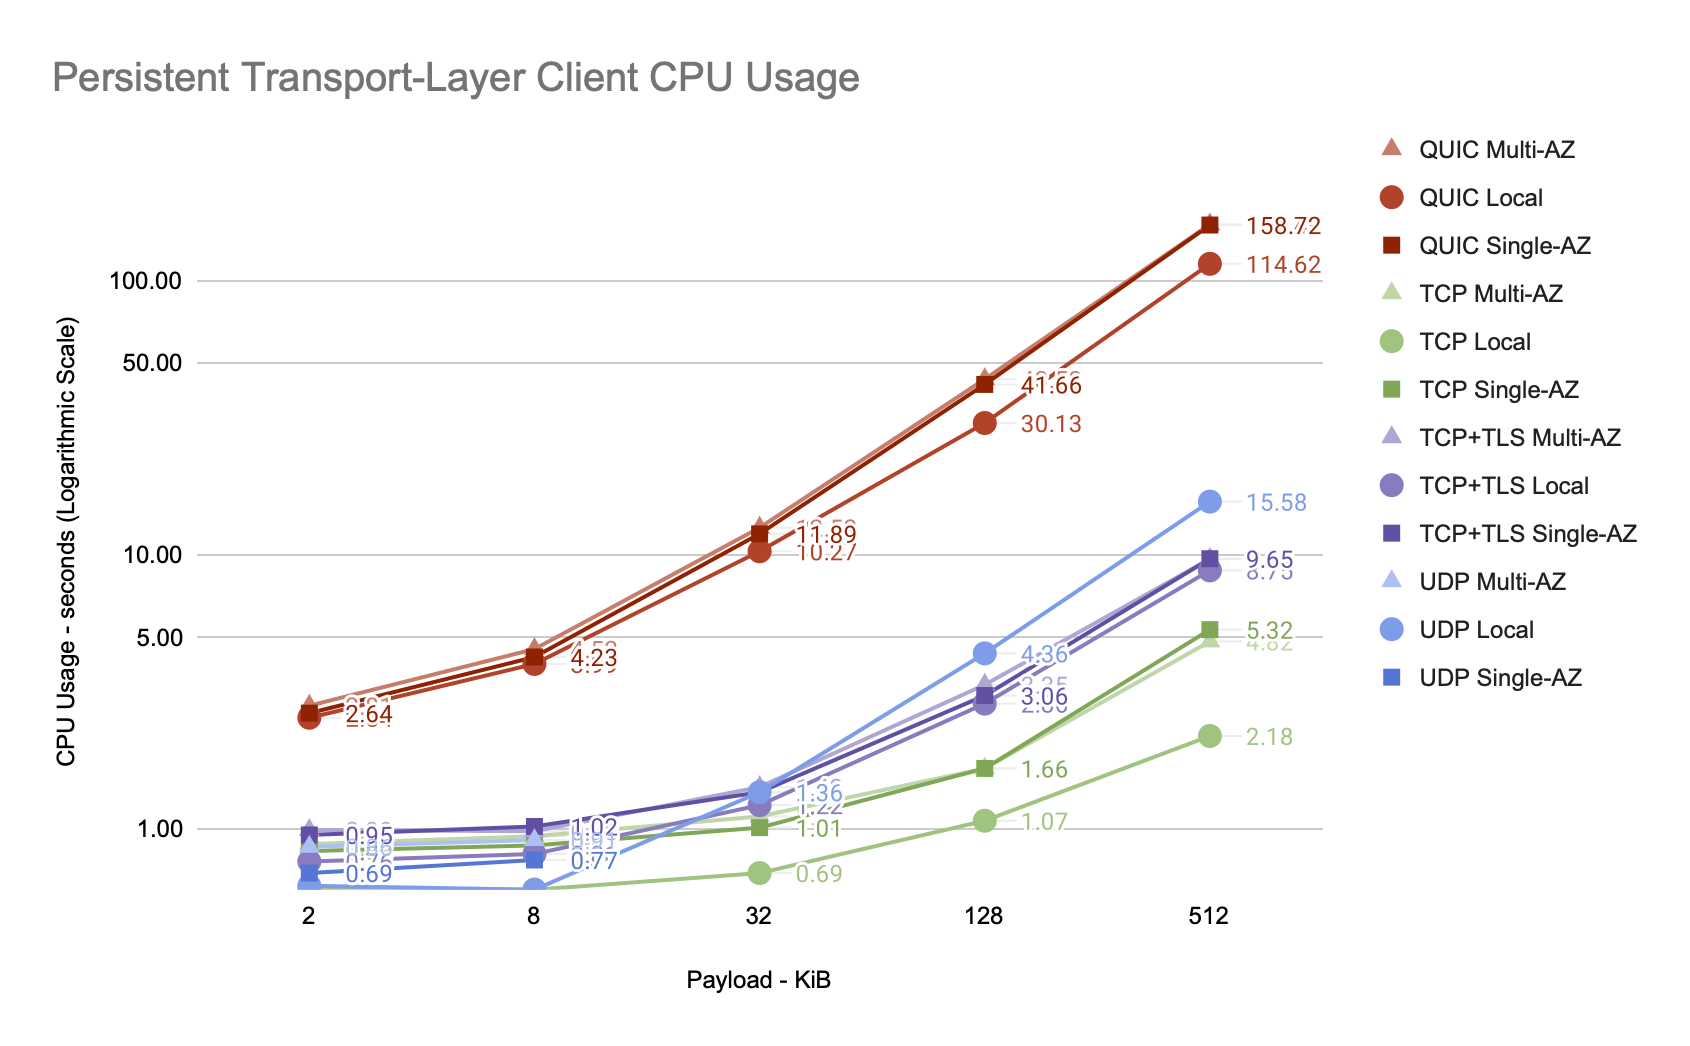
\includegraphics[width=\linewidth]{figures/charts/Persistent Transport-Layer Client CPU Usage.png}
    \caption{Persistent Transport-Layer Client CPU Usage}
    \label{fig:persistent_client_transport_cpu}
\end{figure}

\begin{figure}[h!]
    \centering
    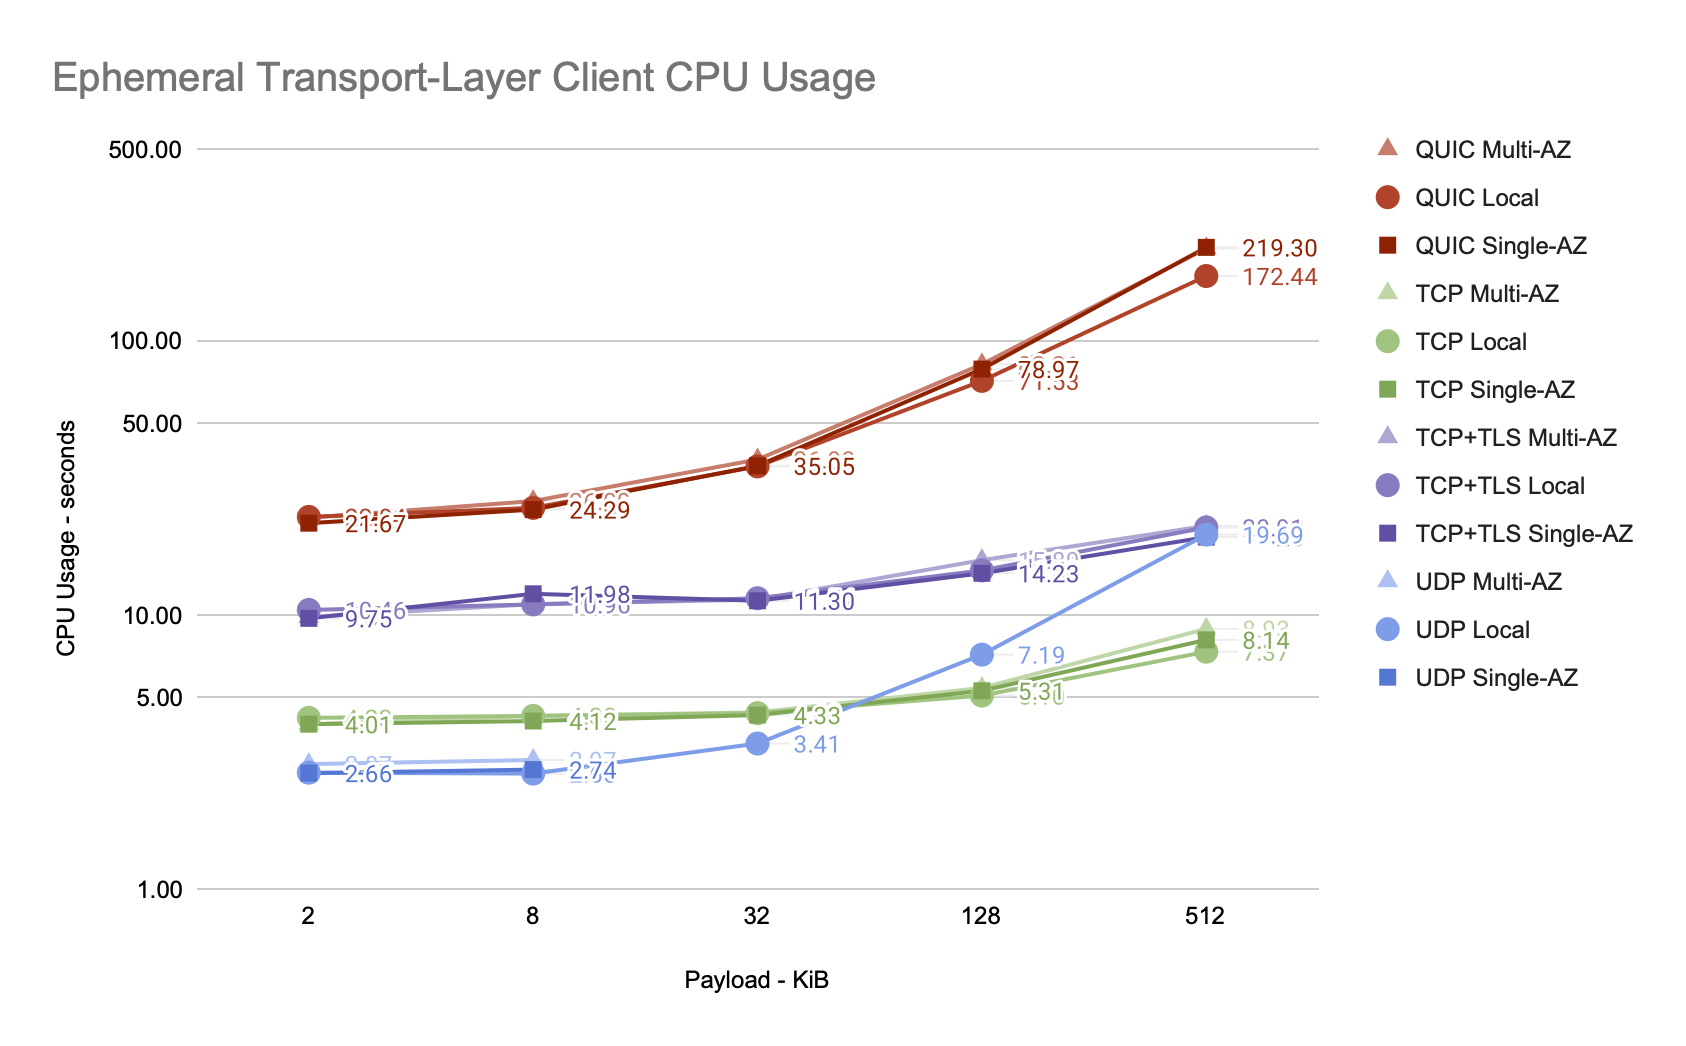
\includegraphics[width=\linewidth]{figures/charts/Ephemeral Transport-Layer Client CPU Usage.png}
    \caption{Ephemeral Transport-Layer Client CPU Usage}
    \label{fig:ephemeral_client_transport_cpu}
\end{figure}

\clearpage

\begin{figure}[h!]
    \centering
    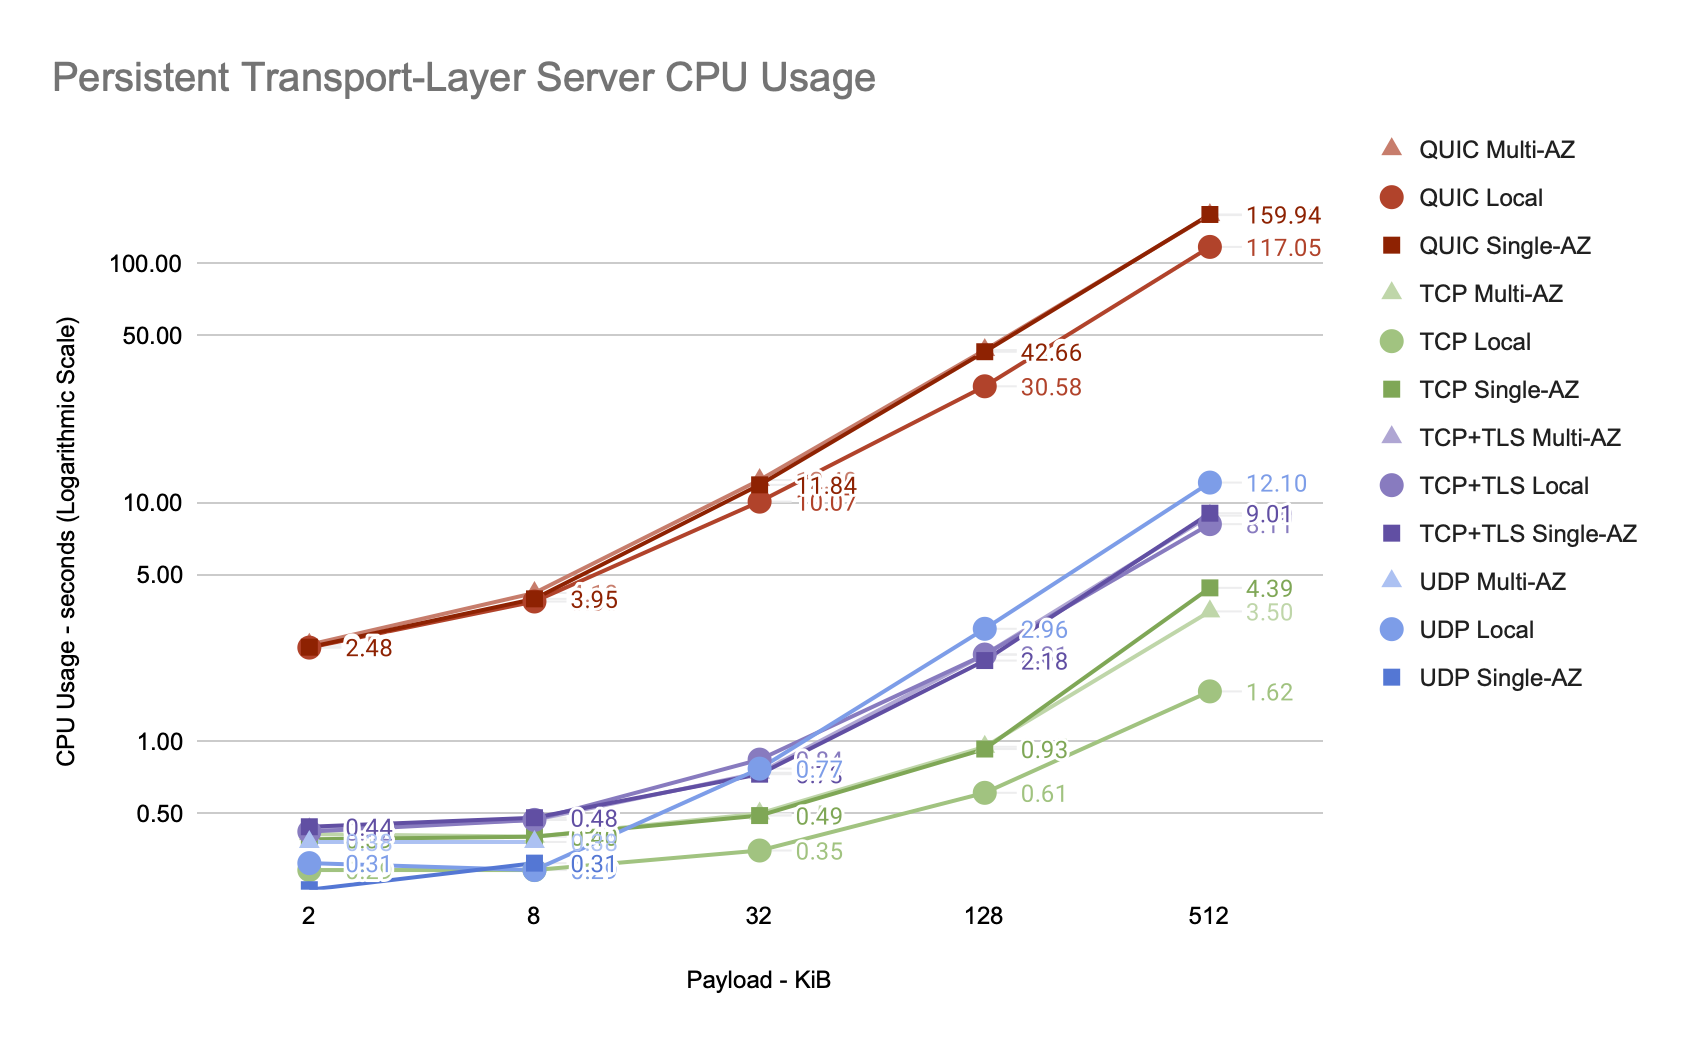
\includegraphics[width=\linewidth]{figures/charts/Persistent Transport-Layer Server CPU Usage.png}
    \caption{Persistent Transport-Layer Server CPU Usage}
    \label{fig:persistent_server_transport_cpu}
\end{figure}

\begin{figure}[h!]
    \centering
    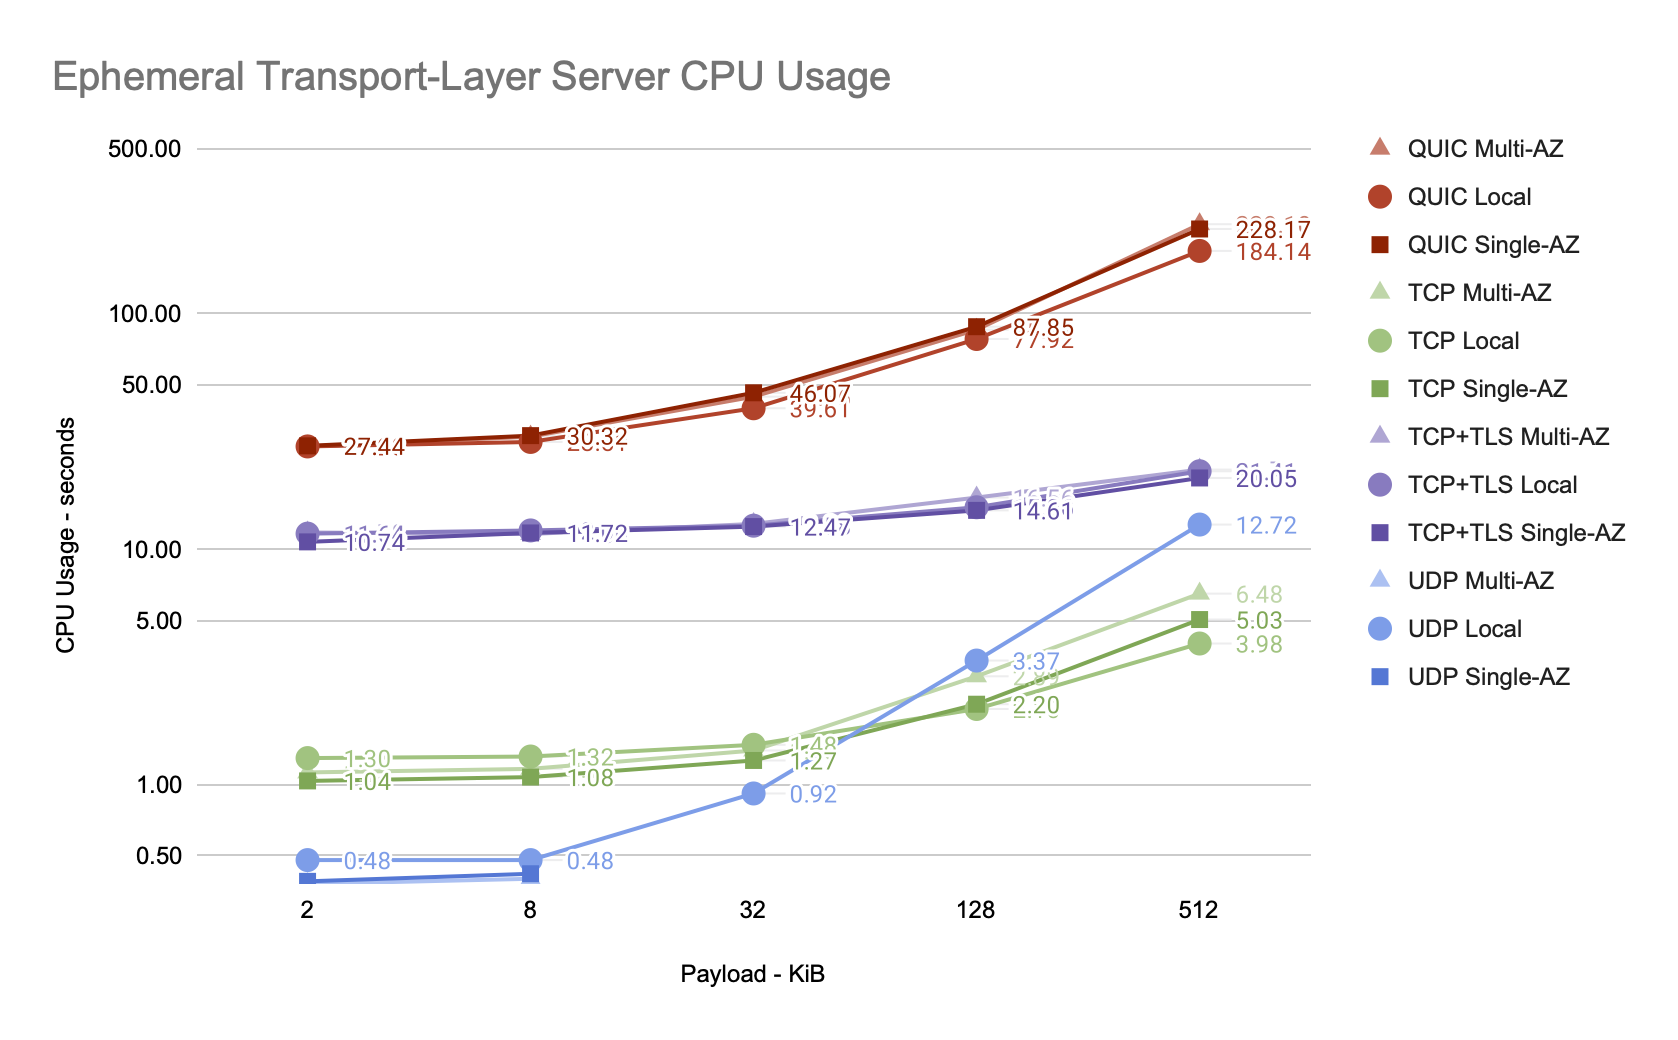
\includegraphics[width=\linewidth]{figures/charts/Ephemeral Transport-Layer Server CPU Usage.png}
    \caption{Ephemeral Transport-Layer Server CPU Usage}
    \label{fig:ephemeral_server_transport_cpu}
\end{figure}

\clearpage
